\documentclass{beamer}
\usepackage{relsize}
\usepackage{color}
\usepackage{rotating}

\usepackage{listings}
\usetheme{CambridgeUS}
%\usepackage{beamerthemesplit} % new
\usepackage{enumitem}
\usepackage{amsmath}                    % See geometry.pdf to learn the layout options.
\usepackage{amsthm}                   % See geometry.pdf to learn the layout options. There
\usepackage{amssymb}                    % See geometry.pdf to learn the layout options.
\usepackage[utf8]{inputenc}
\usepackage{graphicx}
\usepackage[english,bulgarian]{babel}

\lstset{language=C++,
                basicstyle=\ttfamily,
                keywordstyle=\color{blue}\ttfamily,
                stringstyle=\color{red}\ttfamily,
                commentstyle=\color{green}\ttfamily,
                morecomment=[l][\color{magenta}]{\#}
}

\newtheorem{mydef}{Дефиниция}[section]
\newtheorem{lem}{Лема}[section]
\newtheorem{thm}{Твърдение}[section]

\DeclareMathOperator{\restrict}{\upharpoonright}

\setitemize{label=\usebeamerfont*{itemize item}%
  \usebeamercolor[fg]{itemize item}
  \usebeamertemplate{itemize item}}

\setbeamercovered{transparent}



\begin{document}
\title[Увод в програмирането]{Рекурсивни програми}
\frame{\titlepage}


\section{Рекурентни дефиниции}

\begin{frame}
\centerline{Редици, индуктивни дефиниции, индукция, рекурсия}
\end{frame}


\begin{frame}[fragile]
\frametitle{Какво е редица от числа?}

\begin{itemize}
  \item Серия от измервания
\end{itemize}



\begin{figure}[]
  \centering
  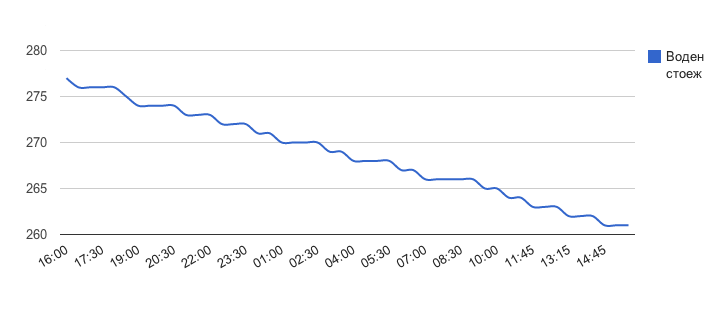
\includegraphics[width=8cm]{images/danube}
  \caption{Нивото на река Дунав в см.}
\end{figure}


\begin{flushleft}
\relscale{0.70}
\begin{tabular}{|c|c|c|c|c}
$a_0=280cm$ & $a_1=275cm$ & $a_2=271cm$ & $a_3=272cm$ & ...
\end{tabular}

\end{flushleft}


\end{frame}



\begin{frame}[fragile]
\frametitle{Описание на феномен?}
\begin{columns}[t]
  \begin{column}{0.6\textwidth}
%\vspace*{-25pt}
    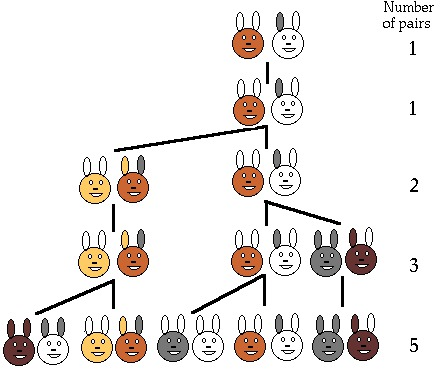
\includegraphics[width=6cm]{images/fib_rabbits}

$a_0=1$


$a_1=1$


$a_{i+2} = a_{i+1} + a_i $
  \end{column}
  \begin{column}{0.4\textwidth}
\vspace*{-150px}

   \begin{center}
   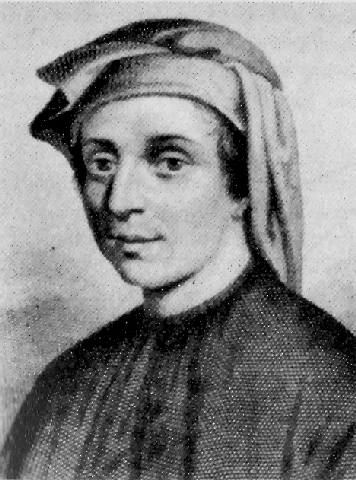
\includegraphics[width=2.4cm]{images/Fibonacci}
    \relscale{0.6}

     Leonardo Fibonacci

     (c. 1170 – c. 1250)
   \end{center}
  \end{column}
\end{columns}




\end{frame}



\begin{frame}[fragile]
\frametitle{Изчисление?}


\begin{columns}[c]
  \begin{column}{0.5\textwidth}

  %\vspace*{-1pt}
    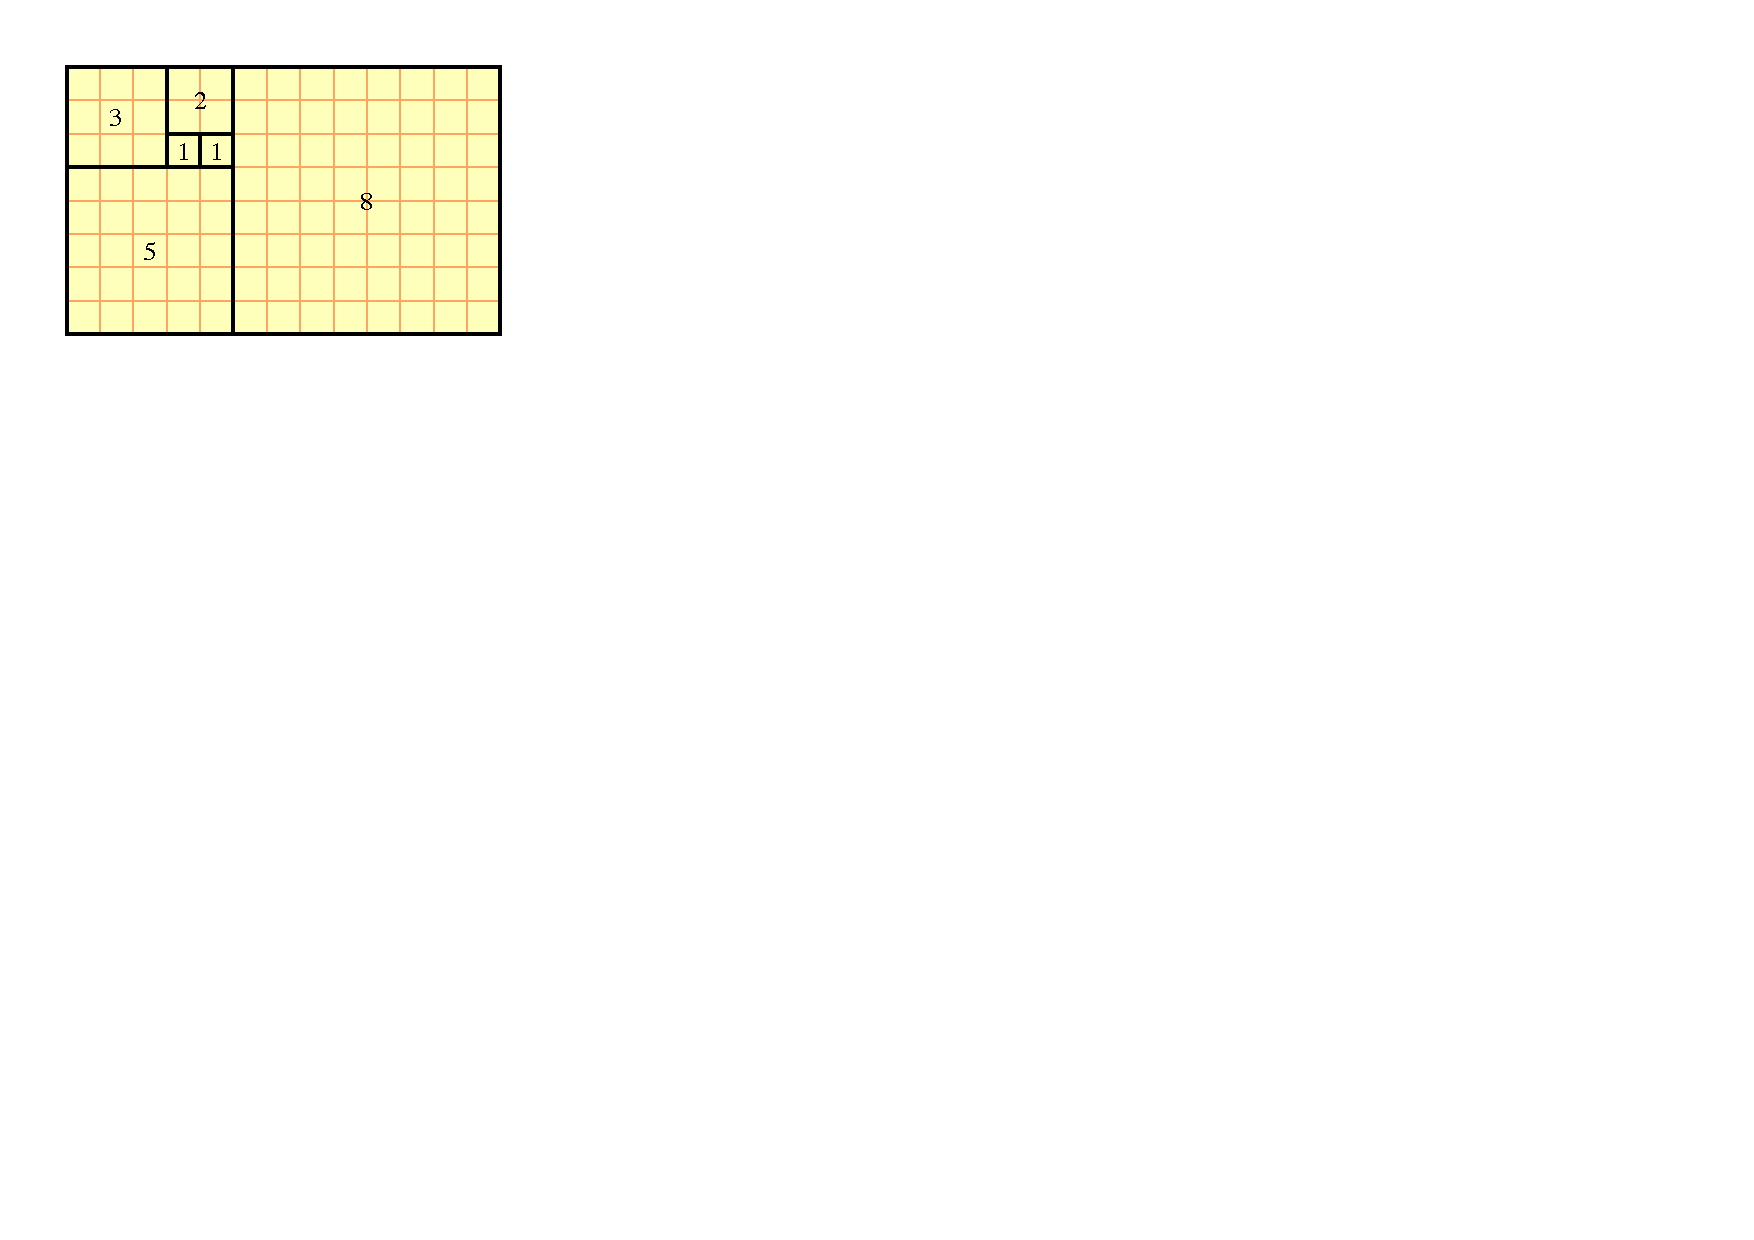
\includegraphics[width=19cm]{images/fib_tiling}
  \end{column}
  \begin{column}{0.5\textwidth}
  \vspace*{250pt}
    \begin{turn}{90}
    \scalebox{1}[1]{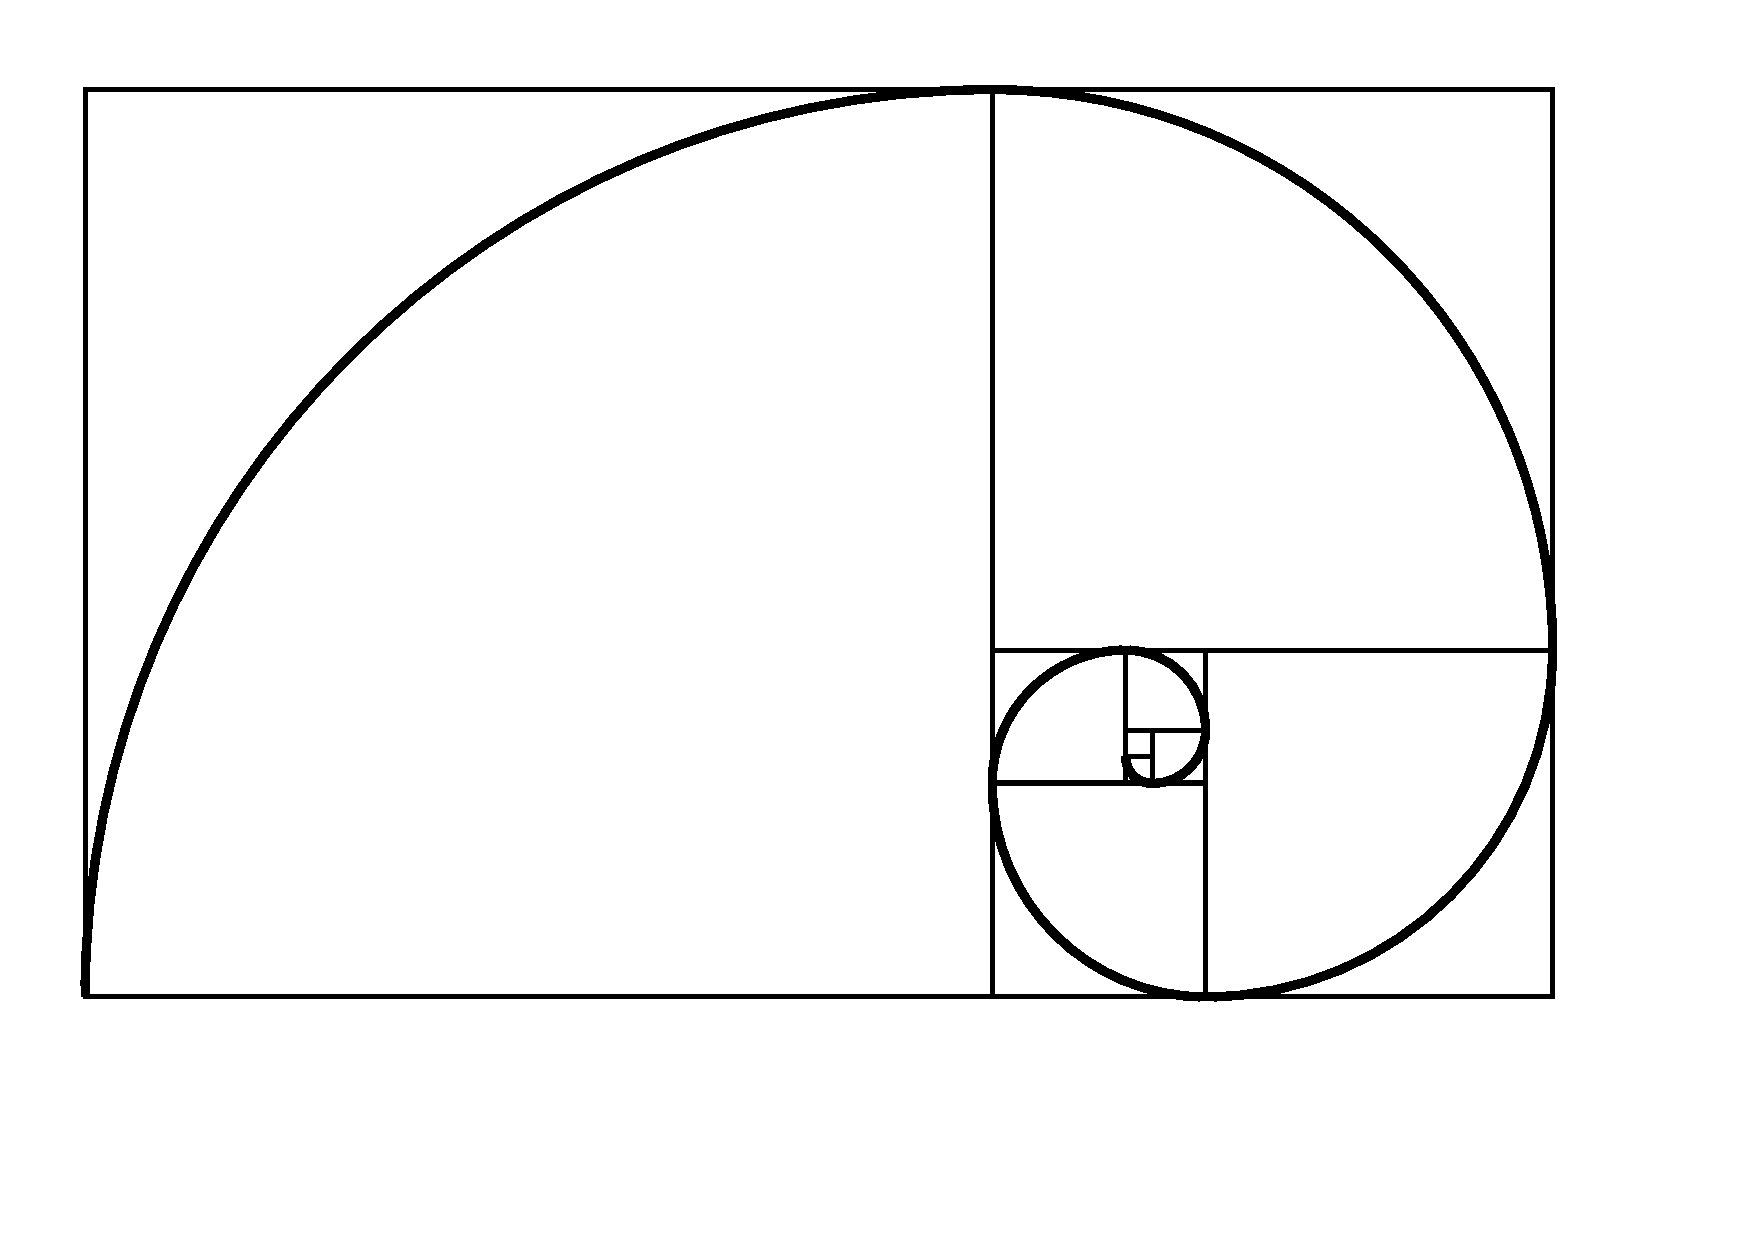
\includegraphics[width=7cm]{images/fib_spiral}}
    \end{turn}
  \end{column}
\end{columns}


\vspace*{-300pt}

$a_0=1$


$a_1=1$


$a_{i+2} = a_{i+1} + a_i $



\end{frame}



\begin{frame}[fragile]
\frametitle{Явна vs. индуктивна дефиниция на елементите на редица}

\begin{center}
$0,2,6,12,20,30,...$
\end{center}

\pause

\begin{itemize}
  \item явна дефиниция
\end{itemize}

\begin{center}
  $\big{\{}a_i\big{\}}_\infty^{i=0}$

  \vspace{10px}

  $a_i = 2 + 4 + ... + 2i = \sum\limits_{k=1,..,i}2k$

\end{center}

\pause

\begin{itemize}
  \item индуктивна дефиниция
\end{itemize}


\begin{center}
  $\big{\{}a_i\big{\}}_\infty^{i=0}$

  \vspace{10px}

  $a_0 = 0$

  $a_i = a_{i-1} + 2i$
\end{center}

a

\end{frame}




\begin{frame}[fragile]
\frametitle{От дефиниция до програма: наивен подход}


\begin{columns}[t]
  \begin{column}{0.6\textwidth}

\relscale{0.70}
\begin{lstlisting}
void print_first_n (int n)
{
  for (int i = 0; i <= n; i++)
  {
    int sum = 0;
    for (int k = 1; k <= i; k++)
    //calculate 2+4+..+2*k
    {
      sum = sum + 2*k;
    }
    cout << "a[" << i << "]="
         << sum << endl;
  }
}
\end{lstlisting}


  \end{column}
  \begin{column}{0.4\textwidth}
\begin{flushleft}
  \relscale{0.95}

  $\big{\{}a_i\big{\}}_\infty^{i=0}$

  \vspace{10px}

  $a_i = 2 + 4 + ... + 2i = \sum\limits_{k=1,..,i}2k$


  \vspace{30px}

  $a_0 = 0$

  $a_1 = 0 + 2$

  $a_2 = 0 + 2 + 4$

  $a_3 = 0 + 2 + 4 + 6$

  ...


\end{flushleft}
  \end{column}
\end{columns}

\end{frame}


\begin{frame}[fragile]
\frametitle{Използваме връзката между членовете на редицата}


\begin{columns}[t]
  \begin{column}{0.7\textwidth}

\relscale{0.75}
\begin{lstlisting}
void print_first_n (int n)
{
  int a_i = 0;

  for (int i = 0; i <= n; i++)
  {
    cout << "a[" << i << "]=" << a_i << endl;

    a_i = a_i + 2*i;
  }
}
\end{lstlisting}


  \end{column}
  \begin{column}{0.3\textwidth}
\begin{flushleft}

  $\big{\{}a_i\big{\}}_\infty^{i=0}$

  \vspace{10px}

  $a_i = a_{i-1} + 2i$

  \vspace{30px}

  $a_0 = 0$

  $a_1 = 0 + 2 = 2$

  $a_2 = 2 + 4 = 6$

  $a_3 = 6 + 6 = 12$


  ...


\end{flushleft}
  \end{column}
\end{columns}

\end{frame}




\begin{frame}[fragile]
\frametitle{Индуктивни дефиниции и рекурсивни функции}


\begin{columns}[t]
  \begin{column}{0.7\textwidth}

\relscale{0.75}
\begin{lstlisting}
int a (int i)
{
  if (i == 0)
    return 0;

  return a(i-1) + 2*i;
}


void print_first_n (int n)
{
  for (int i = 0; i <= n; i++)
  {
    cout << "a["<< i << "]=" << a(i) << endl;
  }
}
\end{lstlisting}


  \end{column}
  \begin{column}{0.3\textwidth}
\begin{flushleft}

  $\big{\{}a_i\big{\}}_\infty^{i=0}$

  \vspace{10px}

  $a_0 = 0$

  $a_i = a_{i-1} + 2i$



\end{flushleft}
  \end{column}
\end{columns}

\end{frame}


\begin{frame}[fragile]
\frametitle{Доказателство по индукция}

\begin{flushleft}
\textbf{Теорема.} За членовете на редицата $\big{\{}a_i\big{\}}_\infty^{i=0}$, дефинирани по следния начин:

\vspace{10px}
$a_0 = 0$

$a_i = a_{i-1} + 2i$
\vspace{10px}

е изпълнено, че $a_i=i(i+1)$, за всяко $n \in \mathcal{N}$.

\vspace{10px}


\textbf{Доказателство.}

\begin{itemize}
  \item За $i=0$ свойството е изпълнено по дефиниция, тъй като $a_0=0=0(0+1)$.
  \item Нека свойството $a_i=i(i+1)$ е изпълнено за някое $i \in \mathcal{N}$. Искаме да покажем, че $a_{i+1}=(i+1)(i+1+1)$ (заместваме $i$ с $i+1$). По дефиниция имаме $a_{i+1} = a_i + 2(i+1)$. Като заместим $a_i$ с $i(i+1)$ (което сме допуснали), получваме

  $a_{i+1} = i(i+1) + 2(i+1) = (i+1)(i+2) $,

  което е търсенето свойство за $a_{i+1}$.
\end{itemize}

\end{flushleft}


\end{frame}



\begin{frame}[fragile]
\frametitle{Прилики / разлики?}



\begin{columns}[t]
  \begin{column}{0.5\textwidth}
\relscale{0.75}
\begin{lstlisting}
int a (int i)
{
  if (i == 0)
    return 0;

  return a(i-1) + 2*i;
}

\end{lstlisting}
  \end{column}
  \begin{column}{0.5\textwidth}
\relscale{0.5}
\begin{flushleft}
\textbf{Теорема.} За членовете на редицата $\big{\{}a_i\big{\}}_\infty^{i=0}$, дефинирани по следния начин:

\vspace{10px}
$a_i = a_{i-1} + 2i$
\vspace{10px}

е изпълнено, че $a_i=i(i+1)$, за всяко $n \in \mathcal{N}$.

\vspace{10px}


\textbf{Доказателство.}

\begin{itemize}
  \item За $i=0$ свойството е изпълнено по дефиниция, тъй като $a_0=0=0(0+1)$.
  \item Нека свойството е изпълнено за $a_{i-1}=(i-1)i$ при $i > 0$. Искаме да покажем, че $a_i=i(i+1)$ (заместваме $i-1$ с $i$). По дефиниция имаме $a_{i} = a_{i-1} + 2i$. Като заместим $a_{i-1}$ с $(i-1)i$ (което сме допуснали), получваме

  $a_{i} = (i-1)i + 2i = i(i-1+2)=i(i+1)$,

  което е търсенето свойство за $a_{i}$.
\end{itemize}

\end{flushleft}


  \end{column}
\end{columns}


\end{frame}

\begin{frame}[fragile]
\frametitle{n-то число на Фибоначи}


\begin{columns}[t]
  \begin{column}{0.7\textwidth}

\relscale{0.75}
\begin{lstlisting}
int fib_n (int n)
{
  if (n == 0)
    return 1;
  if (n == 1)
    return 1;

  return fib_n(n-2) + fin_n(n-1);
}
\end{lstlisting}


  \end{column}
  \begin{column}{0.3\textwidth}
\begin{flushleft}

  $\big{\{}a_i\big{\}}_\infty^{i=0}$

  \vspace{10px}

  $a_0 = 1$

  $a_1 = 1$

  $a_{i+2} = a_{i+1} + a_i$


\end{flushleft}
  \end{column}
\end{columns}

\end{frame}



\begin{frame}[fragile]
\frametitle{n-то число на Фибоначи}

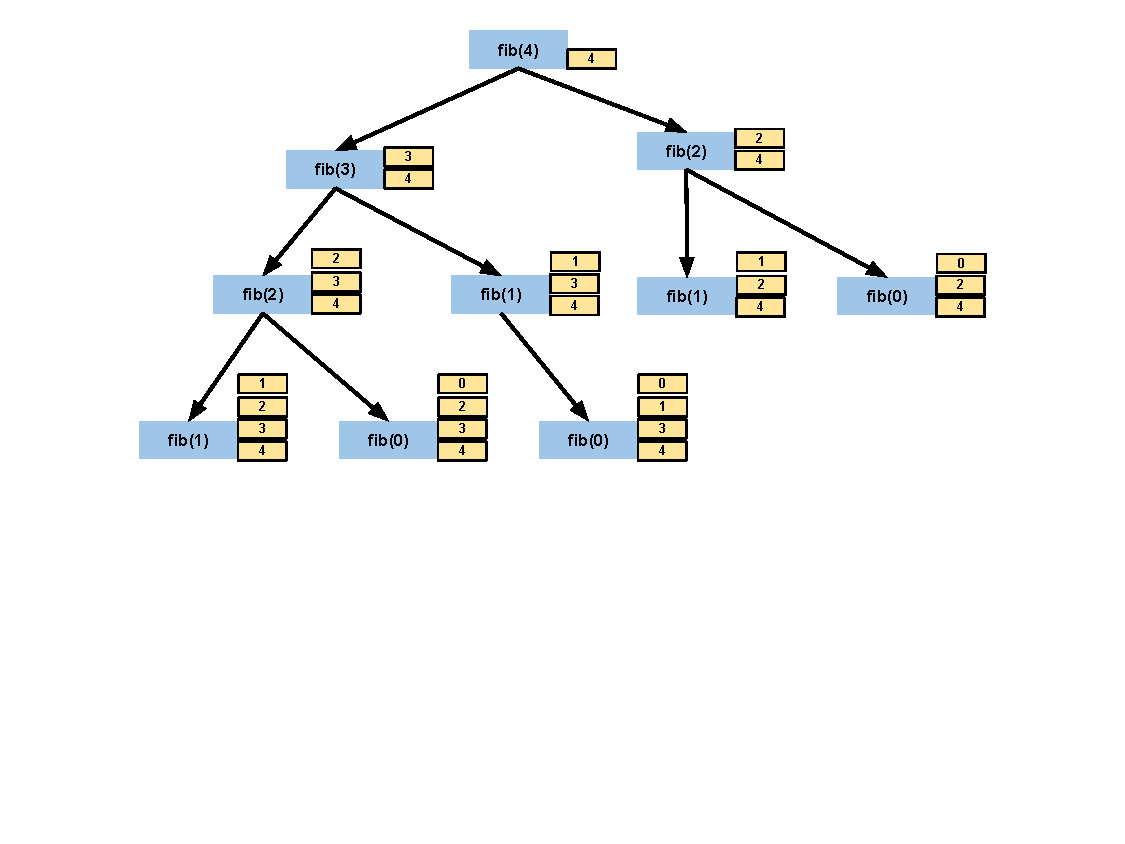
\includegraphics[width=12cm]{images/fib_stack}

\vspace{-100px}

\begin{flushleft}
\relscale{0.55}
\begin{lstlisting}
int fib_n (int n)
{
  if (n <= 1)
    return 1;
  return fib_n(n-2) + fin_n(n-1);
}
\end{lstlisting}
\end{flushleft}


\end{frame}

\begin{frame}
\begin{center}
   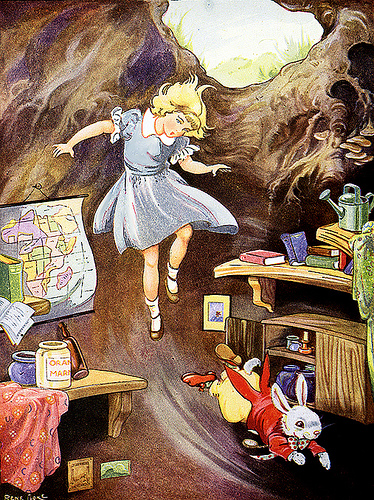
\includegraphics[width=4cm]{images/hole}
\end{center}

\end{frame}



\begin{frame}[fragile]
\frametitle{Факториел}


\begin{columns}[t]
  \begin{column}{0.55\textwidth}

\relscale{0.75}
\begin{lstlisting}
long fact_rec (long n)
{
  if (n <= 1)
    return 1;

  return n*fact_rec(n-1);
}

long fact_iter (long n)
{
  long result = 1;
  while (n > 1)
  {
    result *= n;
    n--;
  }
  return result;
}

\end{lstlisting}


  \end{column}
  \begin{column}{0.45\textwidth}
\begin{flushleft}
  \relscale{0.8}
  $n! = \left\{
        \begin{array}{l l}
          1 & \quad \text{if $n \leq 1$ }\\
    n \times (n-1)! & \quad \text{otherwise}
  \end{array} \right.$

  \vspace{10px}

  $0! = 1$

  $n! = n \times (n-1) \times (n-2) \times ... \times 1$


\end{flushleft}
  \end{column}
\end{columns}

\end{frame}


\begin{frame}[fragile]
\frametitle{Факториел}

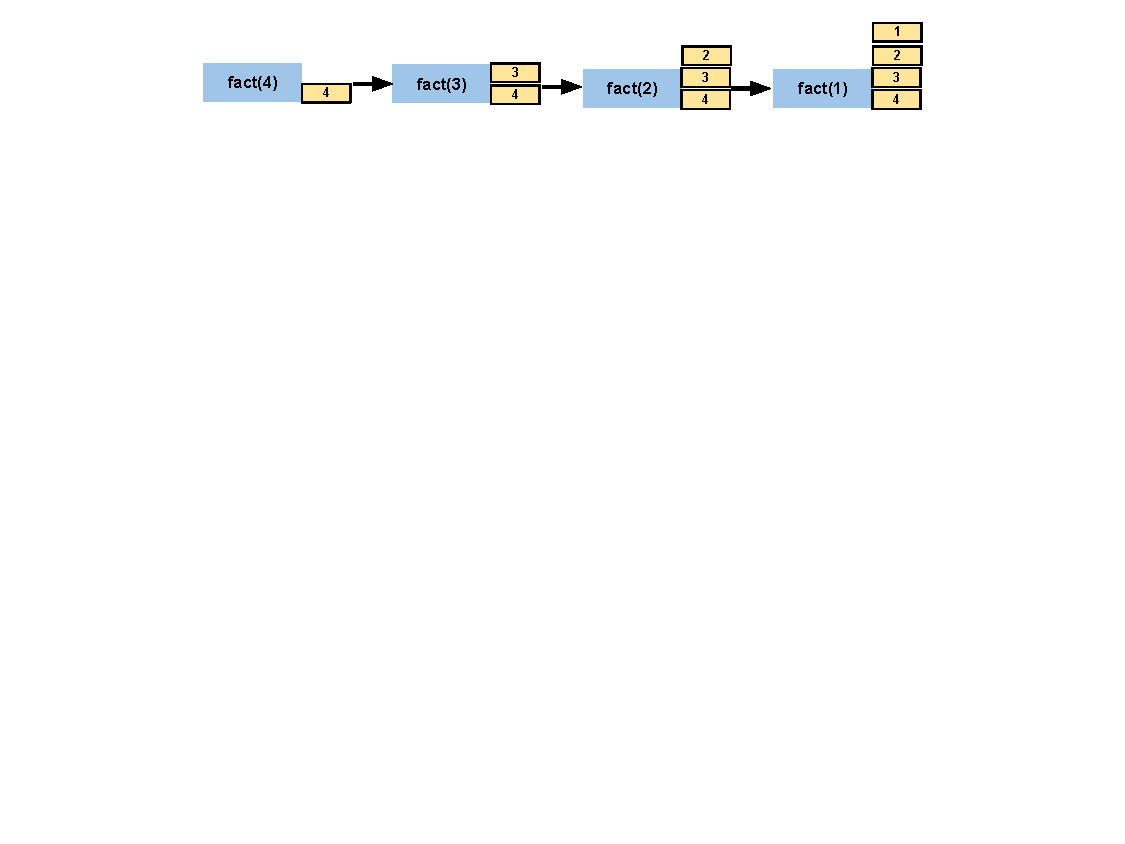
\includegraphics[width=12cm]{images/fact_stack}

\vspace{-150px}

\relscale{0.75}
\begin{lstlisting}
long fact_rec (long n)
{
  if (n <= 1)
    return 1;
  return n*fact_rec(n-1);
}
\end{lstlisting}

\end{frame}



\begin{frame}[fragile]
\frametitle{Сравнение}

\begin{columns}[t]
  \begin{column}{0.5\textwidth}


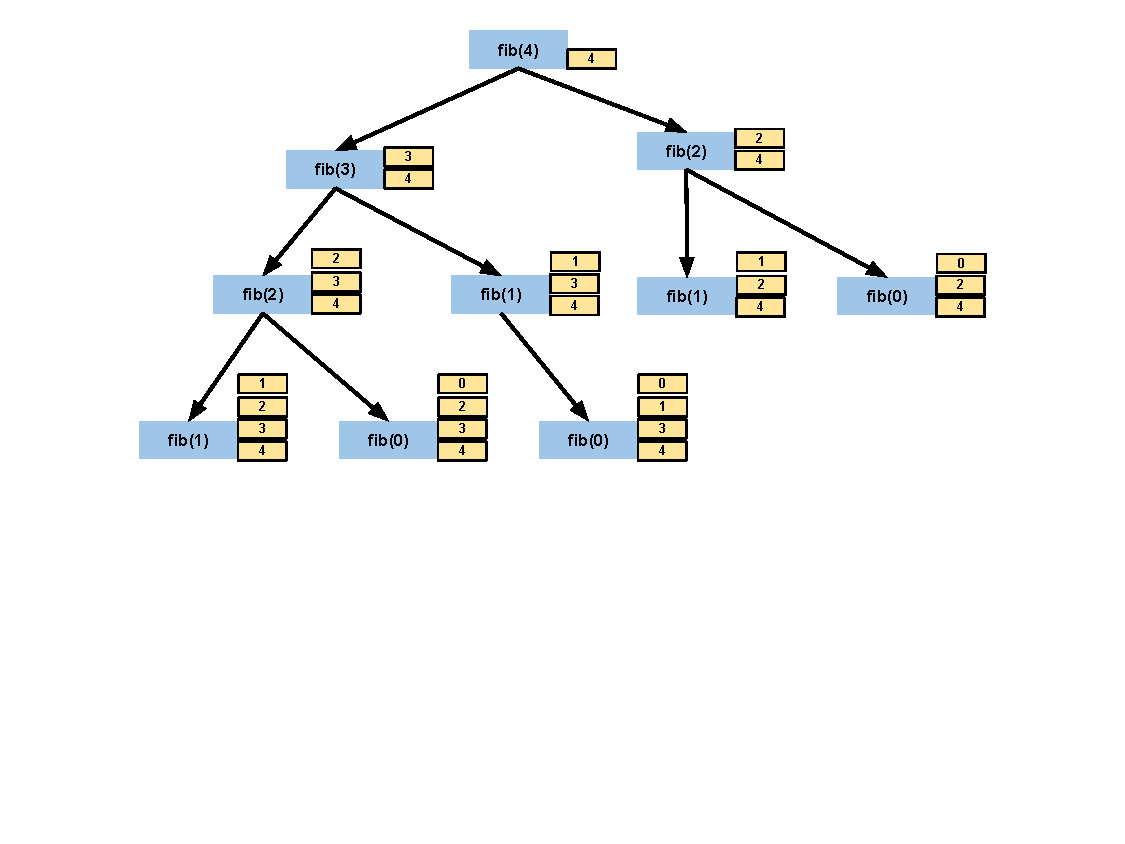
\includegraphics[width=7cm]{images/fib_stack}

\vspace{-50px}

\begin{flushleft}
\relscale{0.55}
\begin{lstlisting}
void fib_n (int n)
{
  if (n <= 1)
    return 1;
  return fib_n(n-2) + fin_n(n-1);
}
\end{lstlisting}
\end{flushleft}


  \end{column}
  \begin{column}{0.5\textwidth}
\vspace{-1px}
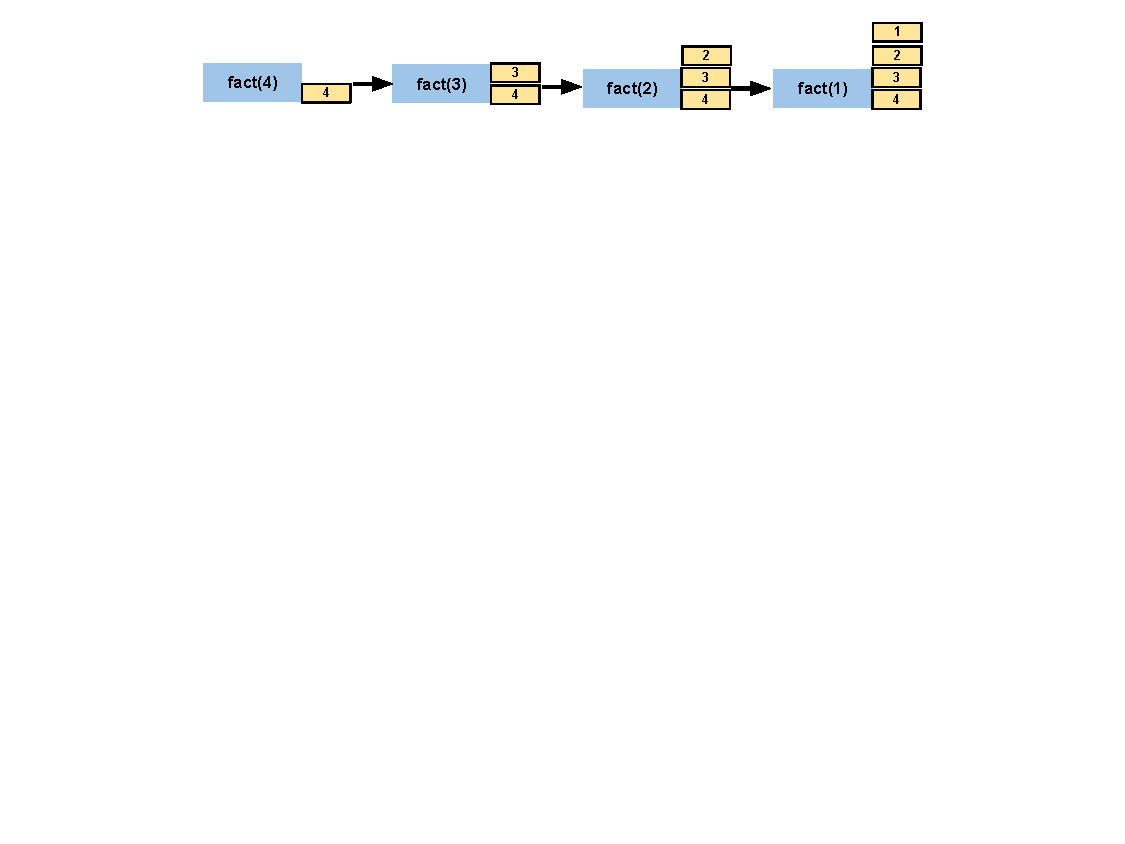
\includegraphics[width=7cm]{images/fact_stack}

\vspace{-40px}

\relscale{0.55}
\begin{lstlisting}
long fact_rec (long n)
{
  if (n <= 1)
    return 1;
  return n*fact_rec(n-1);
}
\end{lstlisting}
  \end{column}
\end{columns}


\end{frame}

\section{Рекурсия}

\begin{frame}
\begin{center}
   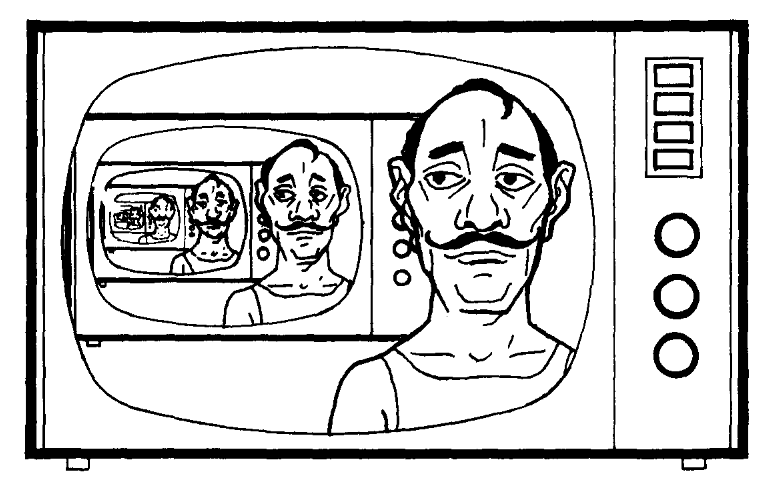
\includegraphics[width=8cm]{images/rec_wirt}
\end{center}
%\vspace{30px}
\relscale{0.5}
\centerline{Wirth.,N.,``Algorithms + Data Structures = Programs'', Prentice Hall,1976}
\end{frame}


\begin{frame}[fragile]
\frametitle{Разлагане на прости делители}

\begin{center}
\begin{center}
\relscale{1.5}
$252=?$
\end{center}

\vspace{15px}

   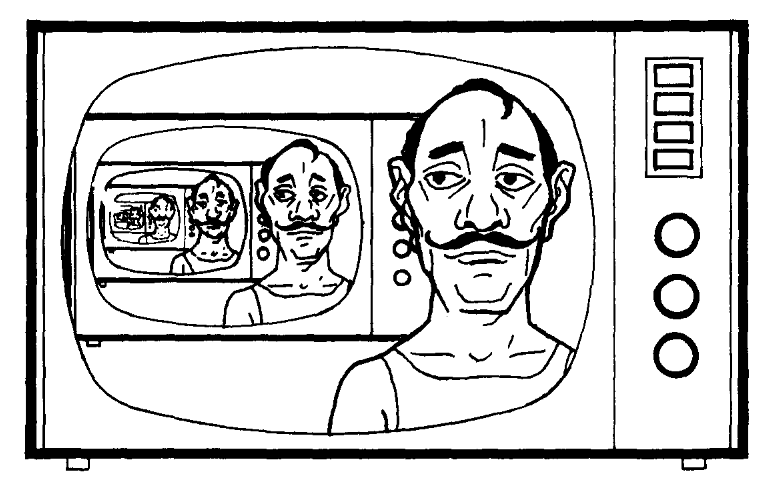
\includegraphics[width=6cm]{images/rec_wirt}
\end{center}

\end{frame}


\begin{frame}[fragile]
\frametitle{Разлагане на прости делители}

\begin{center}
\relscale{1.5}

$252=2.$$\stackrel{126}{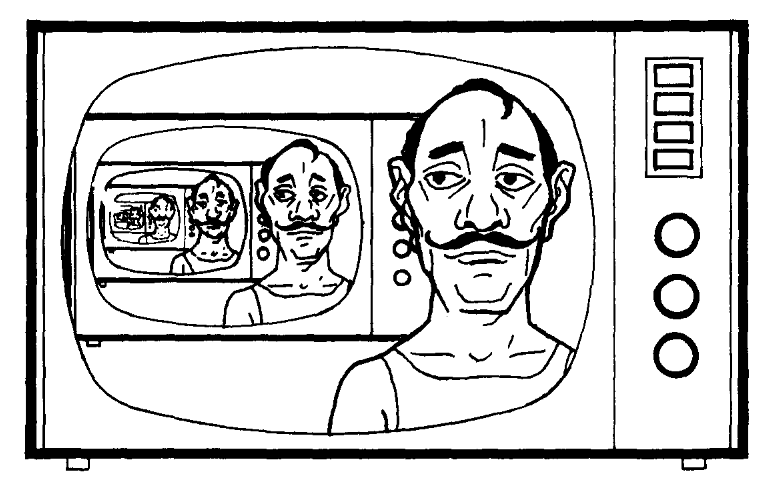
\includegraphics[width=1.5cm]{images/rec_wirt}}$
\end{center}


\end{frame}


\begin{frame}[fragile]
\frametitle{Разлагане на прости делители}


\begin{columns}[t]
  \begin{column}{0.5\textwidth}

\relscale{0.75}
\begin{lstlisting}
void print_divs (int n)
{
  if (n <= 1)
    return;

  int i = 2;
  while (i <= n && n % i != 0)
    i++;

   cout << i << ",";
   print_divs(n/i);
}
\end{lstlisting}


  \end{column}
  \begin{column}{0.5\textwidth}
\begin{flushright}

$351509=17.$$\stackrel{20677}{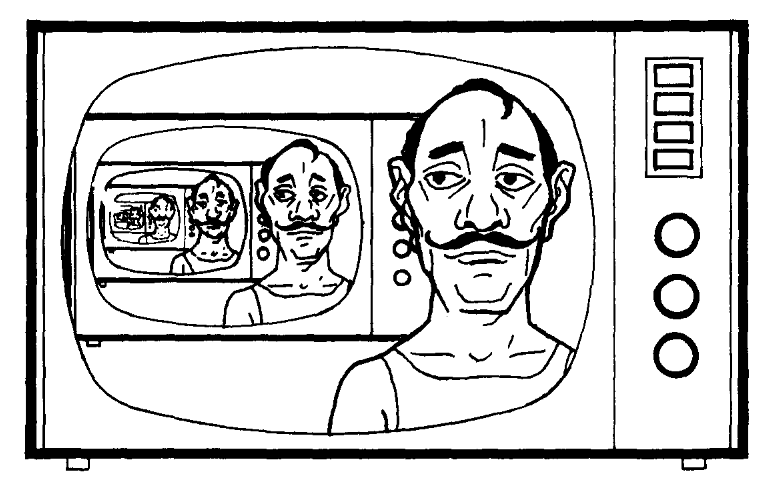
\includegraphics[width=2cm]{images/rec_wirt}}$

$20677=23.$$\stackrel{899}{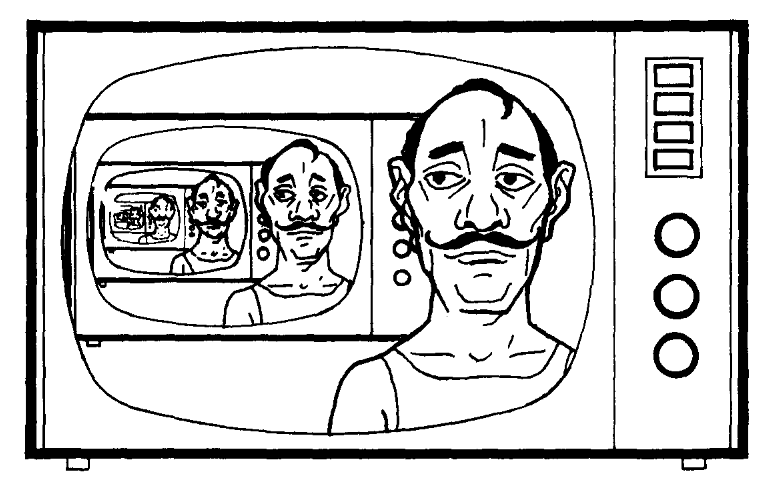
\includegraphics[width=1.6cm]{images/rec_wirt}}$

$899=29.$$\stackrel{31}{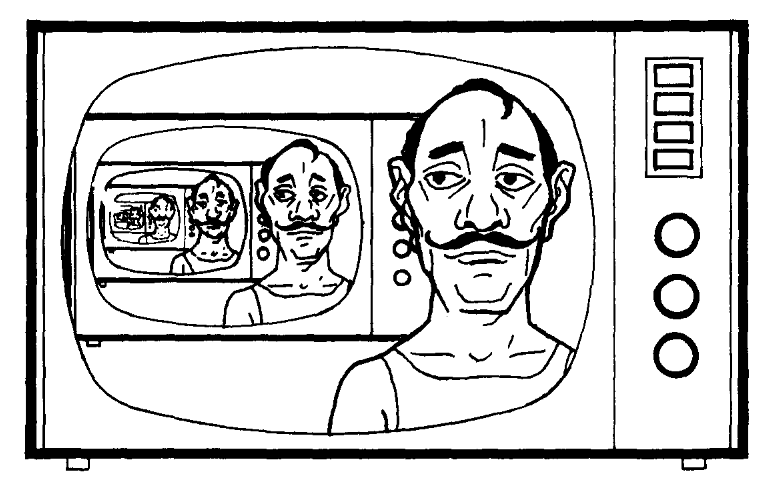
\includegraphics[width=1.2cm]{images/rec_wirt}}$

...


\end{flushright}
  \end{column}
\end{columns}

\end{frame}


\begin{frame}
\begin{center}
   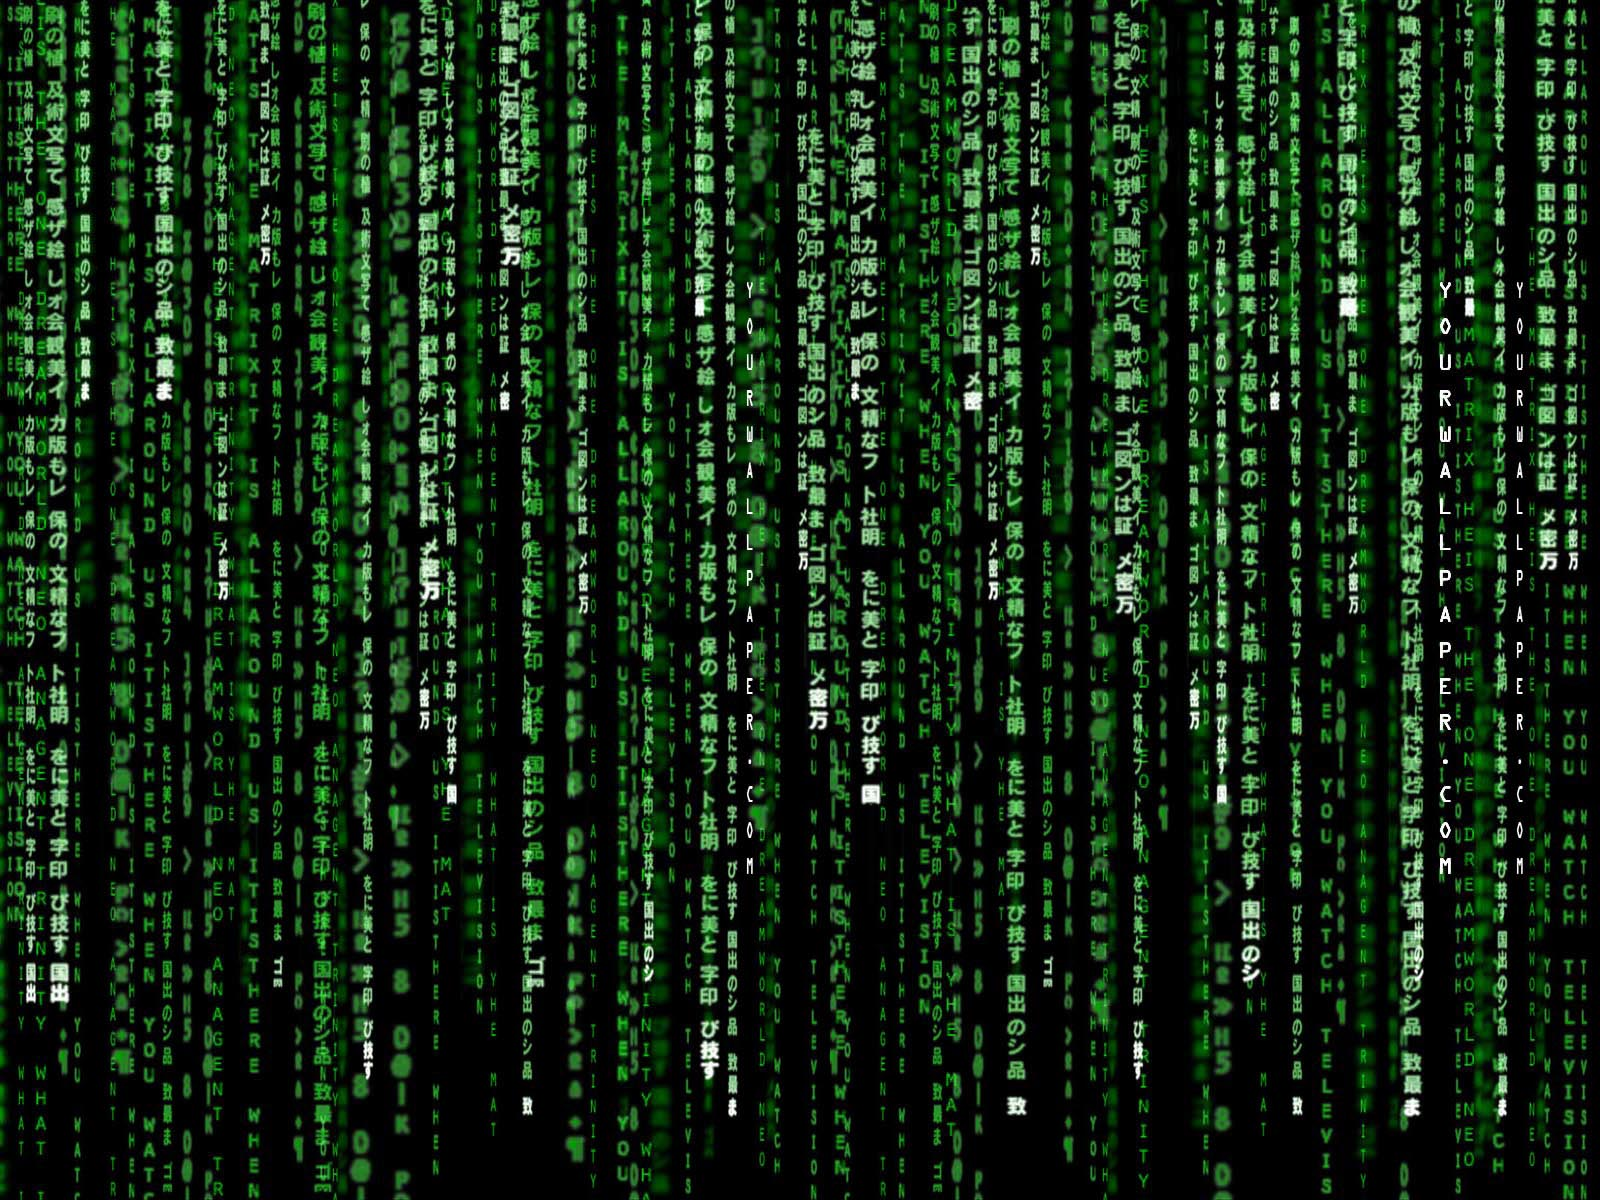
\includegraphics[width=8cm]{images/the_matrix}
\end{center}

\end{frame}


%\begin{frame}
%\begin{center}
%   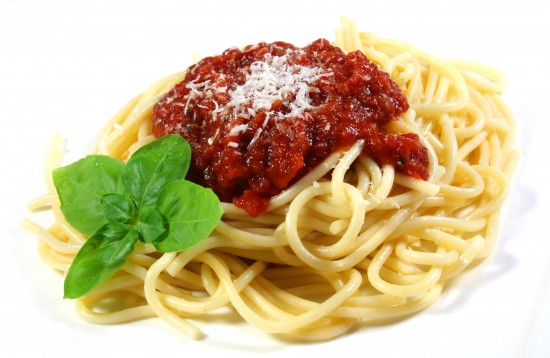
\includegraphics[width=8cm]{images/spaghetti}
%\end{center}
%
%\end{frame}


\section{Рекурсия и масиви}


\begin{frame}[fragile]
\frametitle{Сортиране с рекурсия?}

\begin{center}
   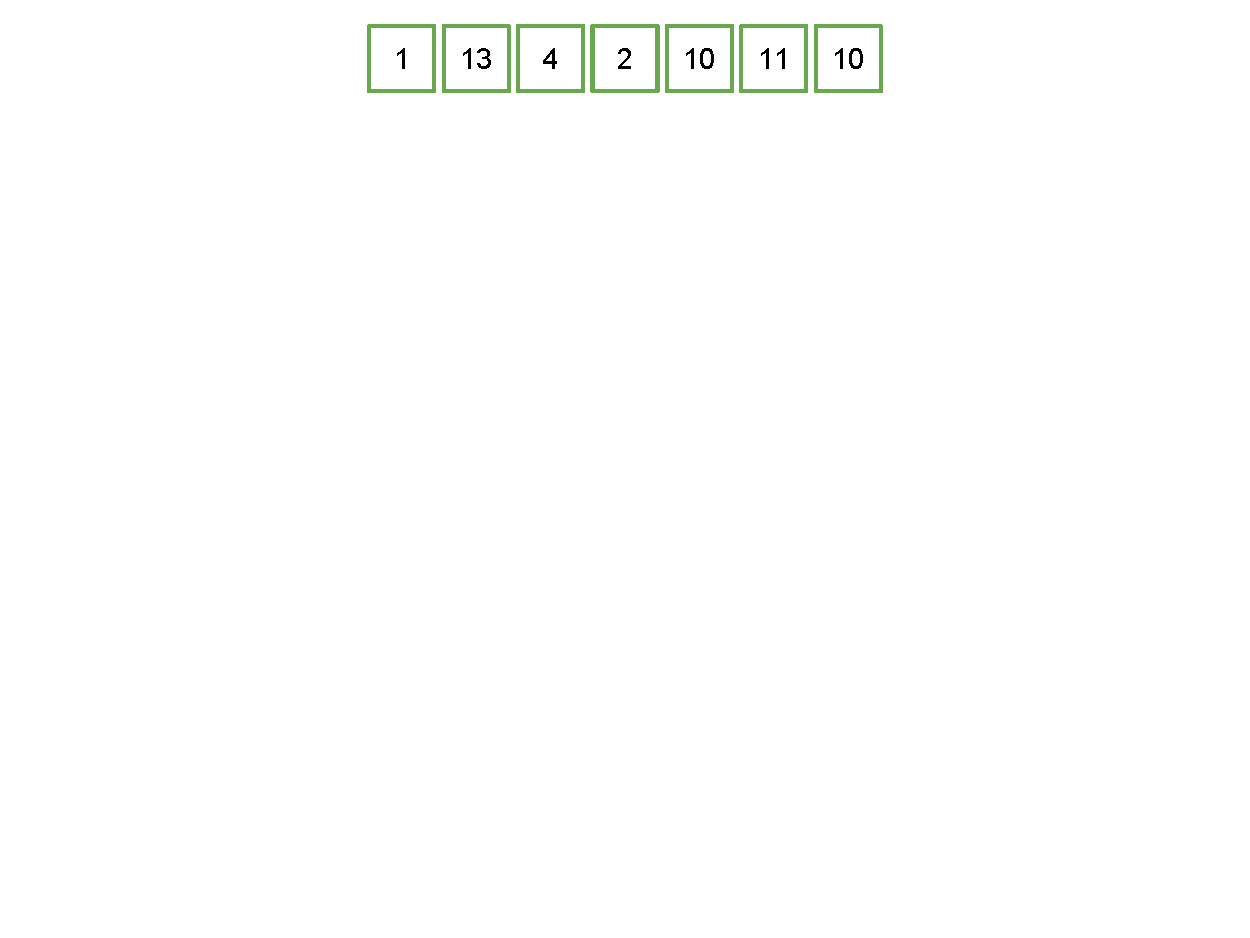
\includegraphics[width=12cm]{images/array_unsorted}

   \vspace{-210px}
   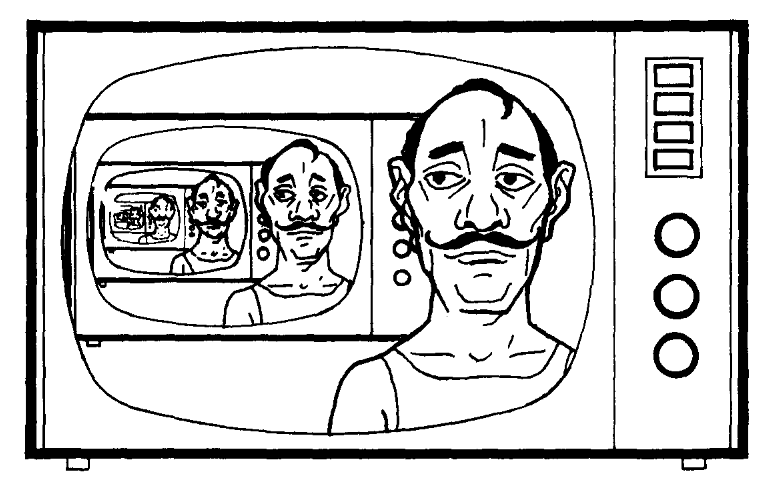
\includegraphics[width=6cm]{images/rec_wirt}
\end{center}

\end{frame}




\begin{frame}[fragile]
\frametitle{Пряка селекция}

\begin{center}
   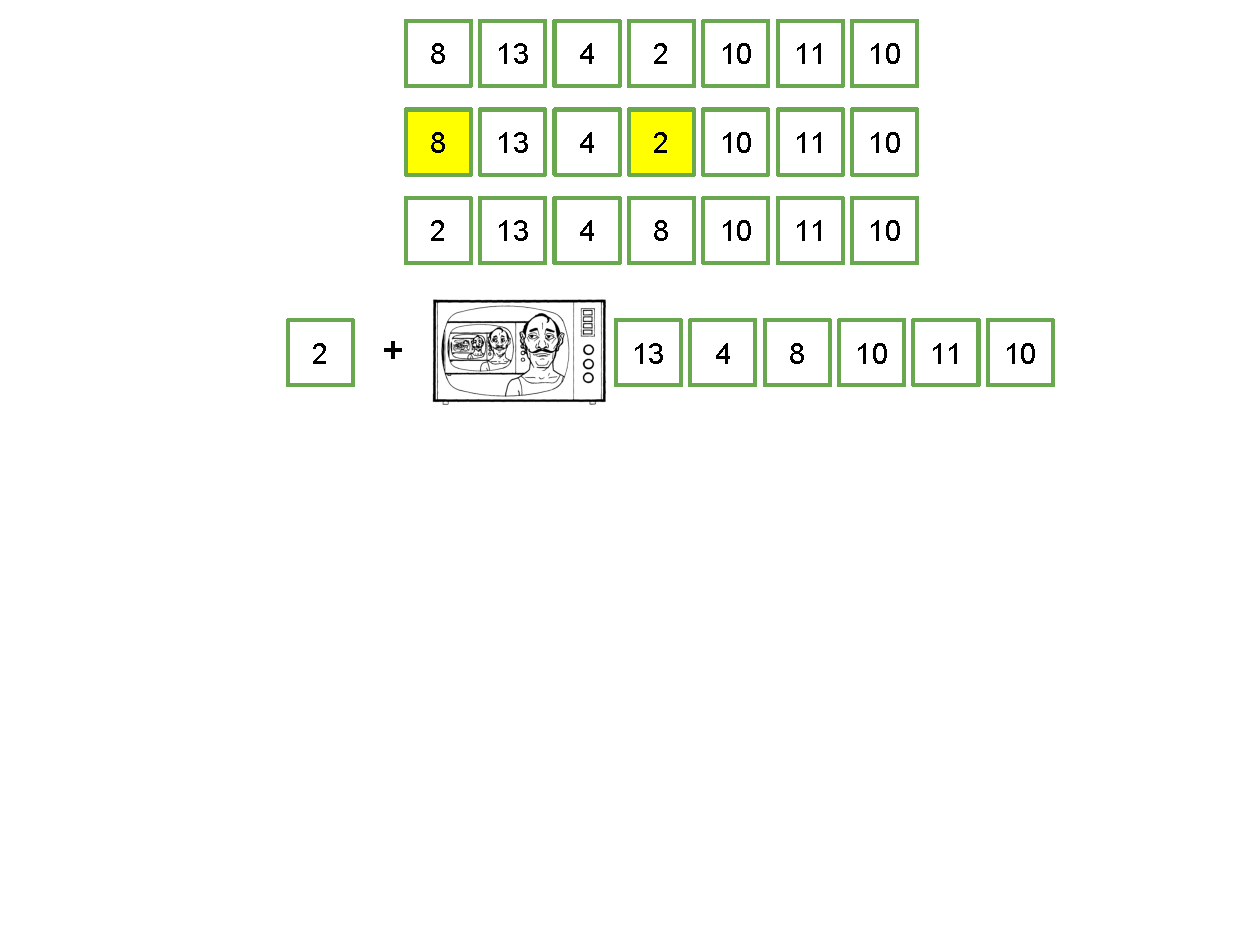
\includegraphics[width=12cm]{images/ssort_rec}
\end{center}

\end{frame}


\begin{frame}[fragile]
\frametitle{Сортиране с пряка селекция}



\begin{columns}[t]
  \begin{column}{0.5\textwidth}

\relscale{0.70}
\begin{lstlisting}
void ssort (int arr[], int n)
{
  if (n <= 1)
    return;

  //find the INDEX OF the minimal
  //element of the array
  int minelIx = 0;
  for (int i = 1; i < n; i++)
    if (arr[minelIx] < arr[i])
      minelIx = i;

  //swap the minimal element and
  //the element at position 0
  int tmp = a[0];
  a[0] = arr[minelIx];
  arr[minelIx] = tmp;

  //sort the "tail" of the array
  ssort (arr+1,n-1);
}
\end{lstlisting}


  \end{column}
  \begin{column}{0.5\textwidth}
\vspace*{-1pt}
\hspace*{-70pt}
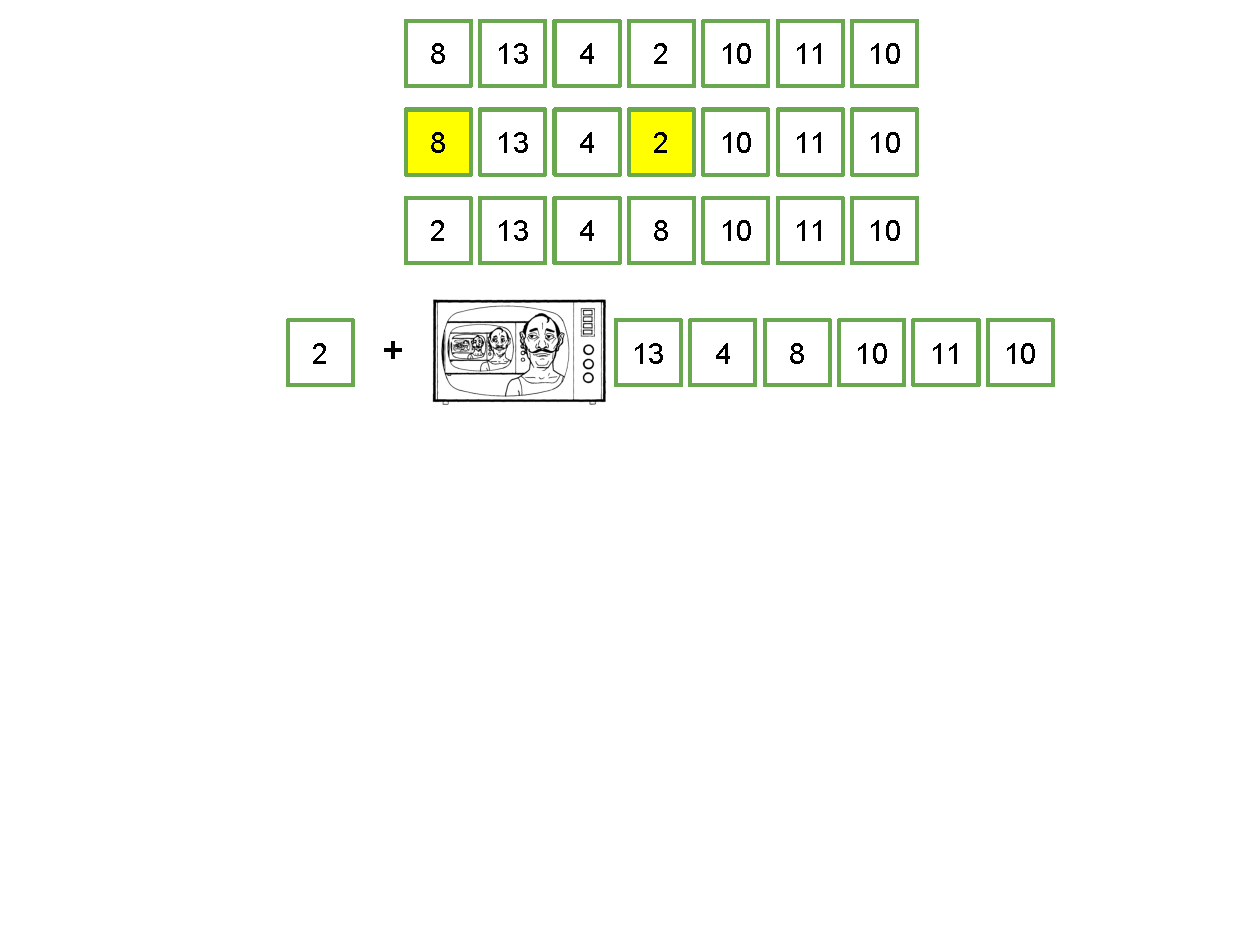
\includegraphics[width=10cm]{images/ssort_rec}

  \end{column}
\end{columns}

\end{frame}



\begin{frame}[fragile]
\frametitle{Да припомним двоичното търсене}



\begin{columns}[t]
  \begin{column}{0.5\textwidth}

\relscale{0.70}
\begin{lstlisting}
bool findrec (int x, int a[], int size)
{
  if (size == 0)
  {
    return false;
  }
  if (size == 1)
  {
    return a[0] == x;
  }
  if (a[size/2] > x)
  {
    return findrec (x,a,size/2);
  }
  if (a[size/2] < x)
  {
    return findrec (x,a+(int)ceil(size/2.0),ceil(size/2.0)-1);
  }
  return true;
}
\end{lstlisting}


  \end{column}
  \begin{column}{0.5\textwidth}
\vspace*{-1pt}
\hspace*{-50pt}
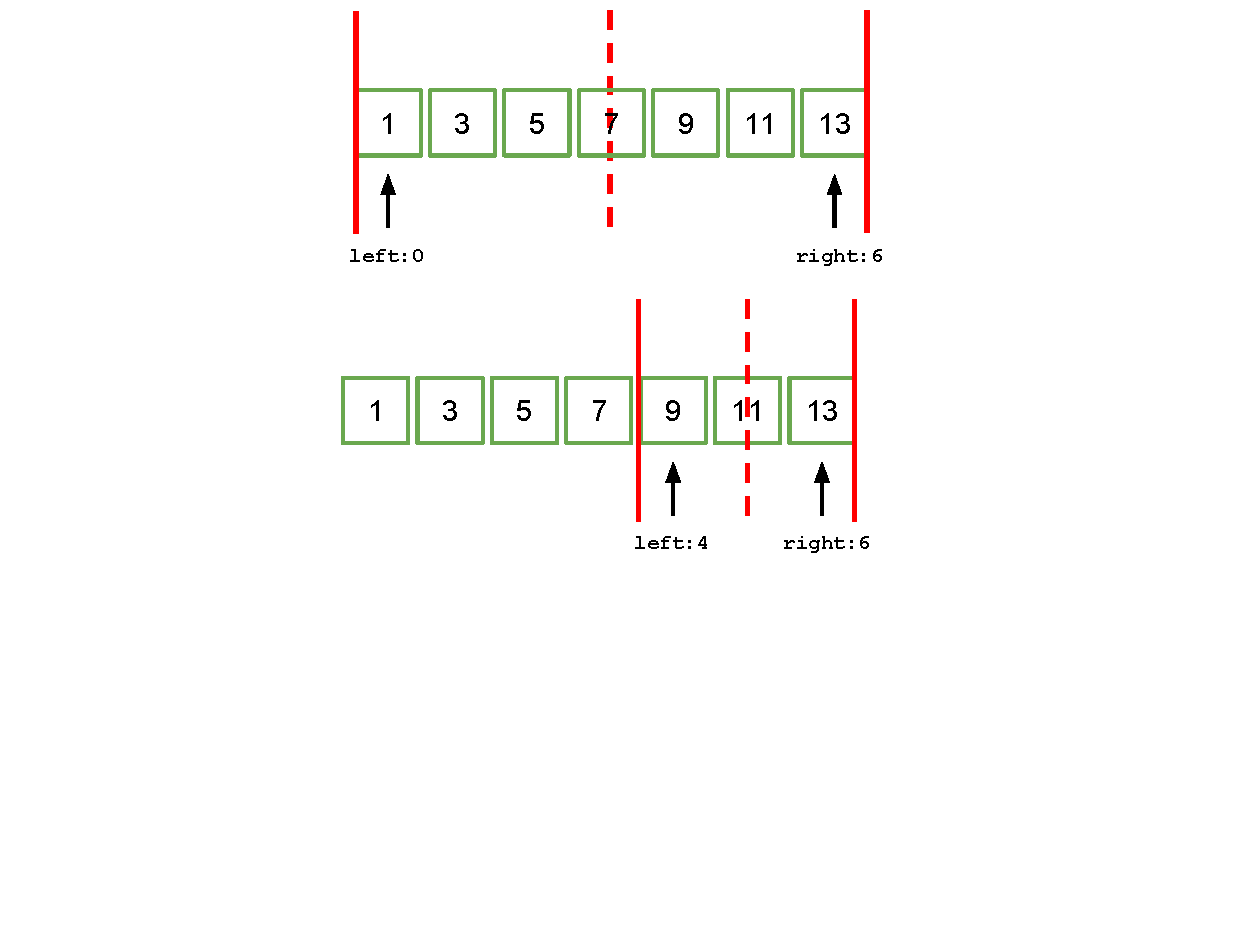
\includegraphics[width=10cm]{images/binsearch_smaller}

  \end{column}
\end{columns}



\end{frame}



\begin{frame}[fragile]
\frametitle{Бързо сортиране}

\begin{center}
   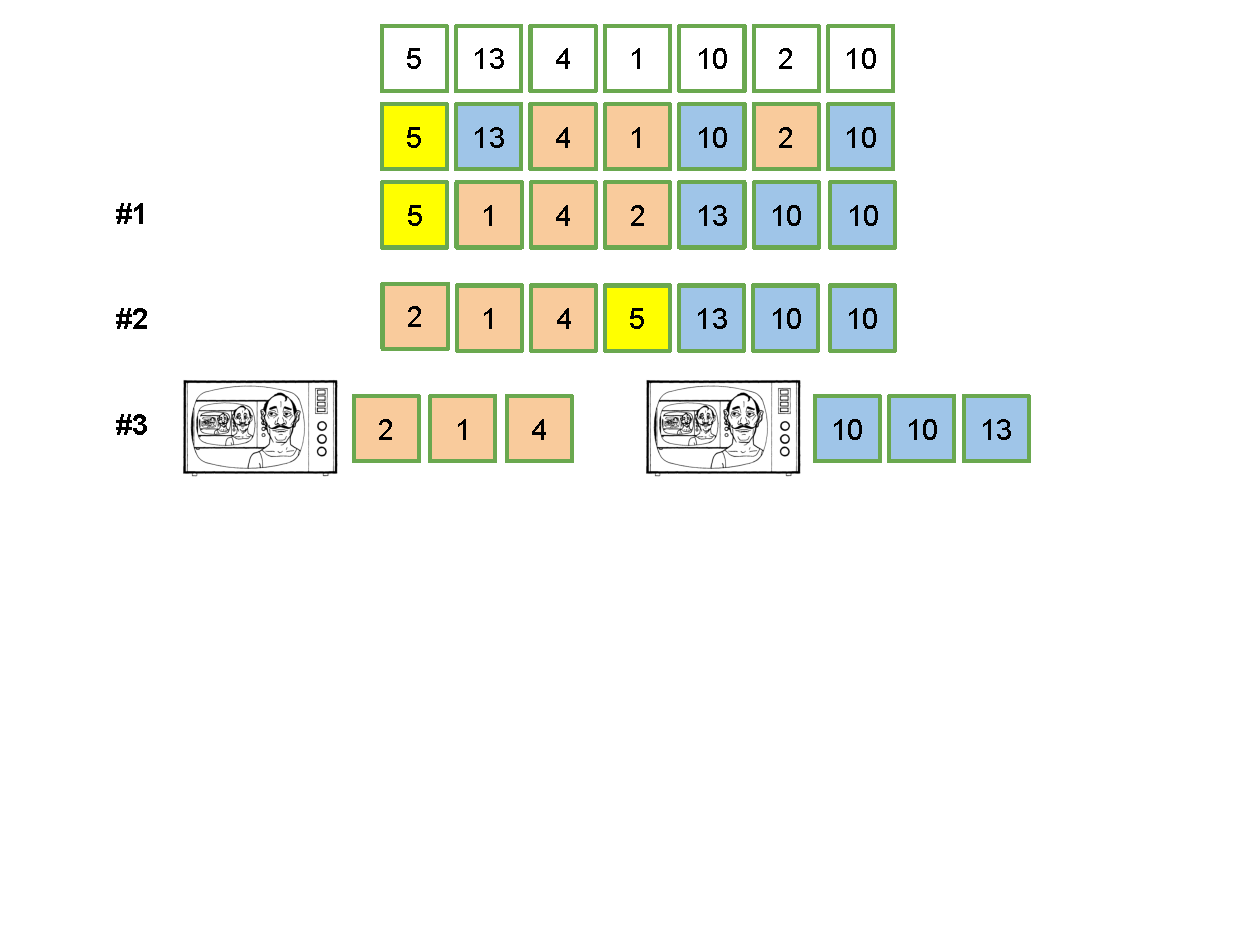
\includegraphics[width=12cm]{images/qsort}
\end{center}

\end{frame}




\begin{frame}[fragile]
\frametitle{Бързо сортиране}



\begin{columns}[t]
  \begin{column}{0.5\textwidth}

\relscale{0.70}
\begin{lstlisting}
bool qsort (int a[], int size)
{
  if (size <= 1)
    return;

  //1
  int nsmaller
    = split (a+1,size-1,a[0]);

  //2
  swap (a[0],a[nsmaller]);

  //3
  qsort(a,nsmaller);
  qsort(a+nsmaller+1,size-nsmaller-1);
}
\end{lstlisting}


  \end{column}
  \begin{column}{0.5\textwidth}
\vspace*{-1pt}
\hspace*{-50pt}
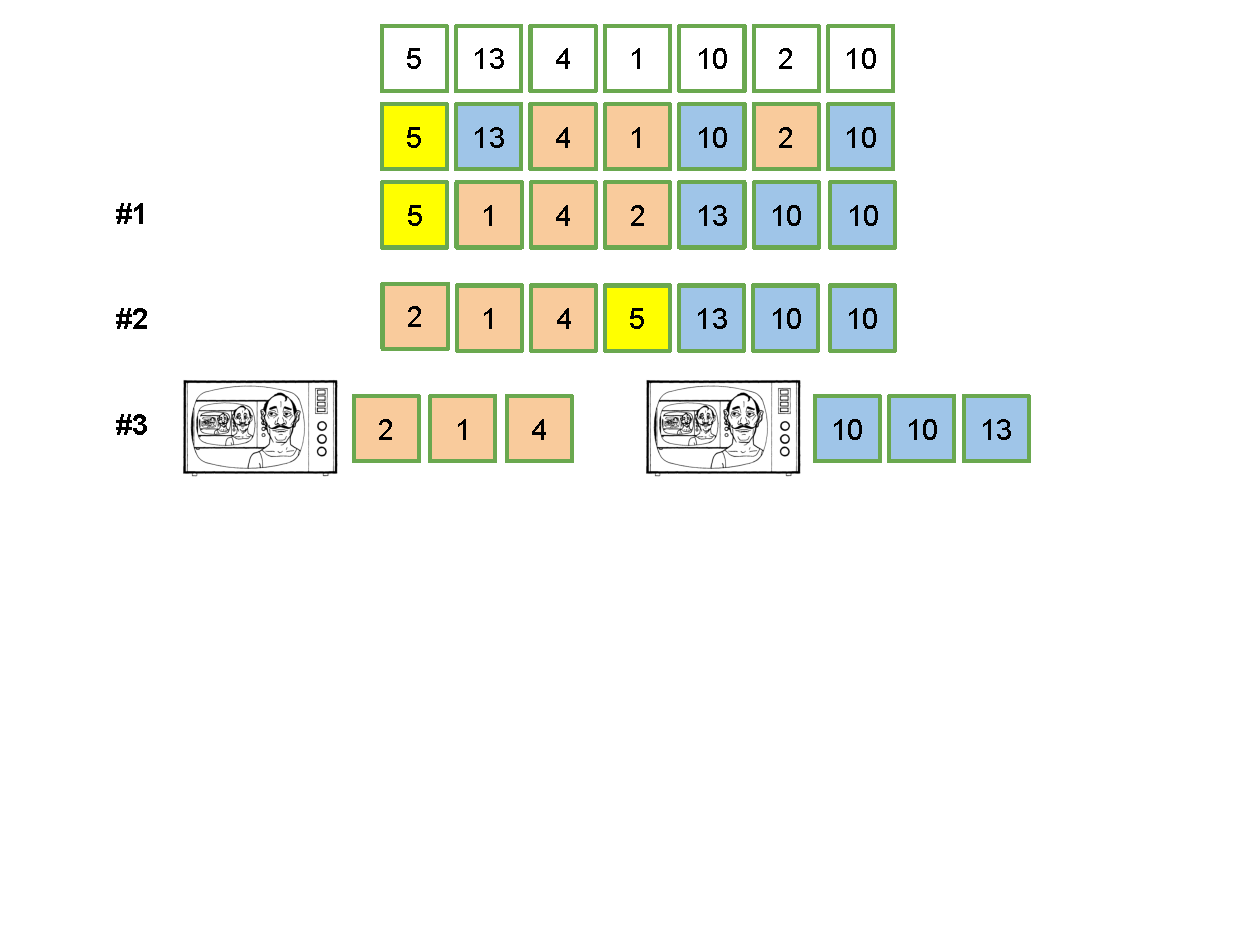
\includegraphics[width=9cm]{images/qsort}

  \end{column}
\end{columns}



\end{frame}



\begin{frame}
\centerline{Благодаря за вниманието!}
\end{frame}


\end{document}


\begin{columns}[t]
  \begin{column}{0.2\textwidth}

  \end{column}
  \begin{column}{0.8\textwidth}

  \end{column}
\end{columns}
